\section{Elementary Cellular Automata}

\begin{frame}{What Are Elementary Cellular Automata?}
  \begin{itemize}
    \item The simplest possible class of cellular automata.
    \item \textbf{1D grid} --- a row of cells, each either 0 (white) or 1 (black).
    \item Each cell's next state depends on its \textbf{current state} and its \textbf{two immediate neighbours}.
    \item There are $2^3 = 8$ possible neighbourhood patterns, each mapped to 0 or 1.
    \item Therefore there are $2^8 = 256$ possible rules, numbered 0--255.
  \end{itemize}
  \vfill
  \begin{center}
    \begin{tikzpicture}[scale=0.5]
      \foreach \x in {0,...,10}{
        \draw (\x,0) rectangle (\x+1,1);
      }
      \fill[primary] (4,0) rectangle (5,1);
      \fill[primary] (5,0) rectangle (6,1);
      \fill[primary] (7,0) rectangle (8,1);
      \draw[thick, secondary] (3,0) rectangle (6,1);
      \node[below, font=\small] at (4.5,-0.2) {neighbourhood};
    \end{tikzpicture}
  \end{center}
\end{frame}

\begin{frame}{The Wolfram Numbering System}
  \small
  Each rule is defined by its output for all 8 possible 3-cell patterns:
  \vfill
  \begin{center}
    \begin{tikzpicture}[scale=0.35]
      % Pattern 111 -> 0
      \fill[primary] (0,1) rectangle (1,2);
      \fill[primary] (1,1) rectangle (2,2);
      \fill[primary] (2,1) rectangle (3,2);
      \draw (1,0) rectangle (2,1);
      \node[below, font=\tiny] at (1.5,-0.3) {111$\to$0};
      % Pattern 110 -> 1
      \fill[primary] (4,1) rectangle (5,2);
      \fill[primary] (5,1) rectangle (6,2);
      \draw (6,1) rectangle (7,2);
      \fill[secondary] (5,0) rectangle (6,1);
      \node[below, font=\tiny] at (5.5,-0.3) {110$\to$1};
      % Pattern 101 -> 1
      \fill[primary] (8,1) rectangle (9,2);
      \draw (9,1) rectangle (10,2);
      \fill[primary] (10,1) rectangle (11,2);
      \fill[secondary] (9,0) rectangle (10,1);
      \node[below, font=\tiny] at (9.5,-0.3) {101$\to$1};
      % Pattern 100 -> 0
      \fill[primary] (12,1) rectangle (13,2);
      \draw (13,1) rectangle (14,2);
      \draw (14,1) rectangle (15,2);
      \draw (13,0) rectangle (14,1);
      \node[below, font=\tiny] at (13.5,-0.3) {100$\to$0};
      % Pattern 011 -> 1
      \draw (16,1) rectangle (17,2);
      \fill[primary] (17,1) rectangle (18,2);
      \fill[primary] (18,1) rectangle (19,2);
      \fill[secondary] (17,0) rectangle (18,1);
      \node[below, font=\tiny] at (17.5,-0.3) {011$\to$1};
      % Pattern 010 -> 1
      \draw (20,1) rectangle (21,2);
      \fill[primary] (21,1) rectangle (22,2);
      \draw (22,1) rectangle (23,2);
      \fill[secondary] (21,0) rectangle (22,1);
      \node[below, font=\tiny] at (21.5,-0.3) {010$\to$1};
      % Pattern 001 -> 1
      \draw (24,1) rectangle (25,2);
      \draw (25,1) rectangle (26,2);
      \fill[primary] (26,1) rectangle (27,2);
      \fill[secondary] (25,0) rectangle (26,1);
      \node[below, font=\tiny] at (25.5,-0.3) {001$\to$1};
      % Pattern 000 -> 0
      \draw (28,1) rectangle (29,2);
      \draw (29,1) rectangle (30,2);
      \draw (30,1) rectangle (31,2);
      \draw (29,0) rectangle (30,1);
      \node[below, font=\tiny] at (29.5,-0.3) {000$\to$0};
    \end{tikzpicture}
  \end{center}
  \vfill
  Example: \textbf{Rule 110} has outputs $0,1,1,0,1,1,1,0$ $\Rightarrow$ binary $01101110$ $= 110$.
  \vfill
  \begin{itemize}
    \item Stephen Wolfram systematically studied all 256 rules.
    \item Despite their simplicity, some rules produce remarkably complex behaviour.
  \end{itemize}
\end{frame}

\begin{frame}{Visualising Elementary CA}
  \begin{itemize}
    \item Start with a single black cell in the centre of a row.
    \item Apply the rule to produce the next row.
    \item Stack rows top to bottom --- time flows downward.
    \item The resulting 2D image reveals the rule's behaviour.
  \end{itemize}
  \vfill
  \begin{center}
    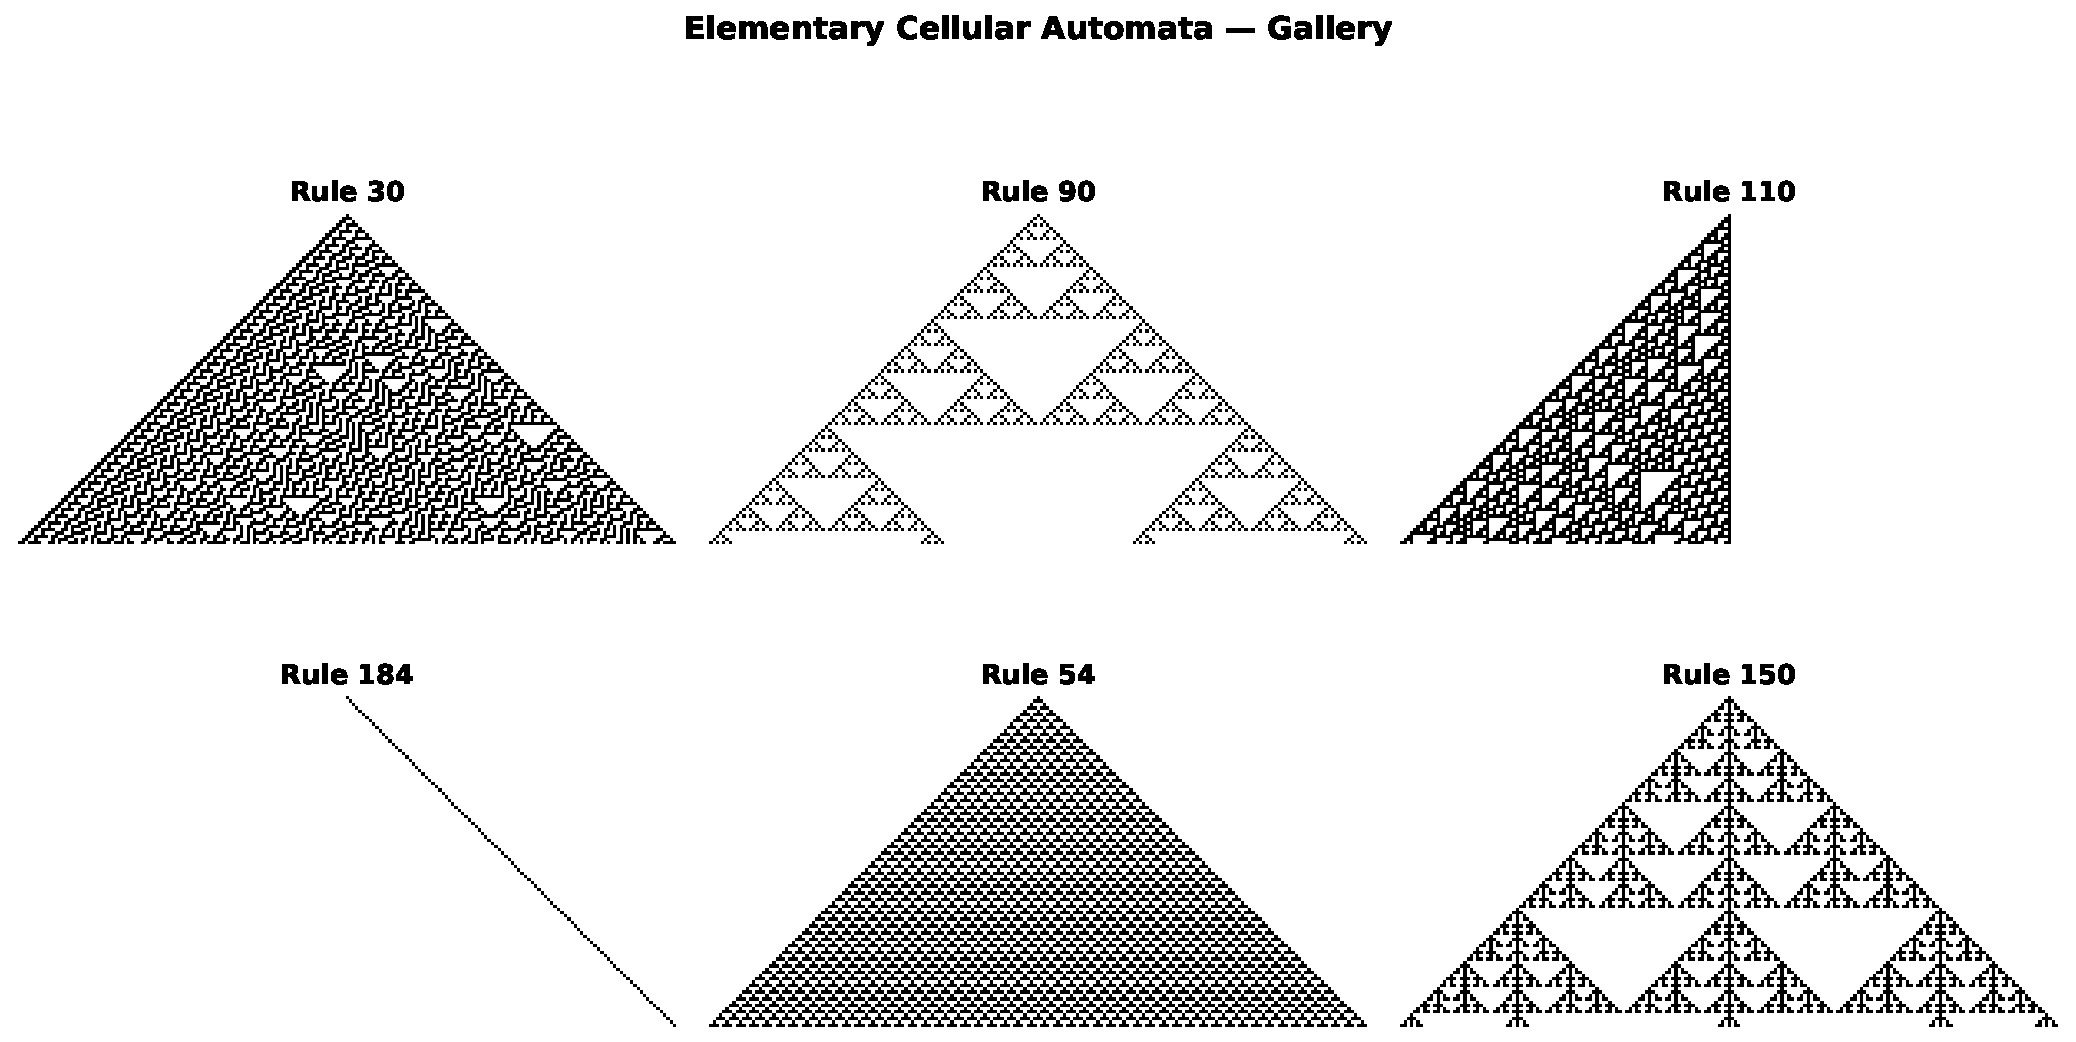
\includegraphics[width=0.85\textwidth]{images/eca_gallery.pdf}
  \end{center}
\end{frame}

\begin{frame}{Wolfram's Four Classes}
  \begin{enumerate}
    \item \textbf{Class I} --- Evolution leads to a \textbf{uniform} state (e.g.\ Rule 0, Rule 32).
    \item \textbf{Class II} --- Evolution leads to \textbf{periodic} or \textbf{stable} structures (e.g.\ Rule 4, Rule 108).
    \item \textbf{Class III} --- Evolution leads to \textbf{chaotic}, aperiodic behaviour (e.g.\ Rule 30, Rule 45).
    \item \textbf{Class IV} --- Evolution leads to \textbf{complex localised structures} (e.g.\ Rule 110, Rule 54).
  \end{enumerate}
  \pause
  \vfill
  \begin{itemize}
    \item Class IV is the most interesting --- it sits at the \textbf{edge of chaos}.
    \item \textbf{Rule 110} has been proven to be \textbf{Turing complete} --- it can perform any computation.
  \end{itemize}
\end{frame}

\begin{frame}{Rule 30 --- Chaos from Simplicity}
  \begin{columns}
    \column{0.5\textwidth}
    \begin{center}
      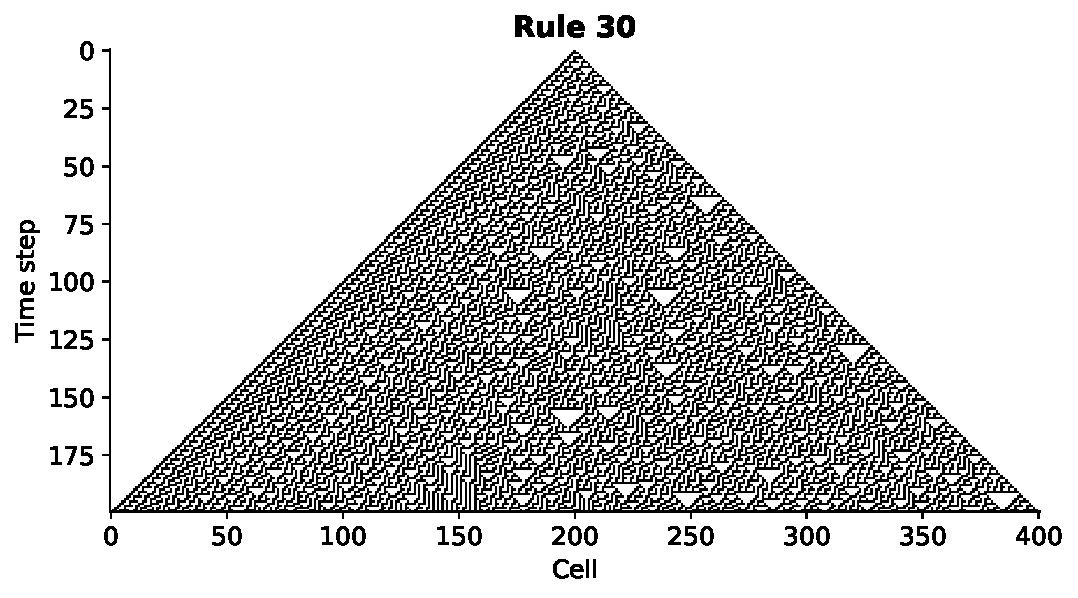
\includegraphics[width=\textwidth]{images/eca_rule30.pdf}
    \end{center}
    \column{0.5\textwidth}
    \begin{itemize}
      \item Rule 30 produces \textbf{chaotic} patterns from a single black cell.
      \item The central column passes statistical tests for \textbf{randomness}.
      \item Wolfram used it as a random number generator in \textit{Mathematica}.
      \item The pattern appears on the shell of the \textit{Conus textile} sea snail.
    \end{itemize}
  \end{columns}
\end{frame}

\begin{frame}{Rule 110 --- Complexity and Computation}
  \begin{columns}
    \column{0.5\textwidth}
    \begin{center}
      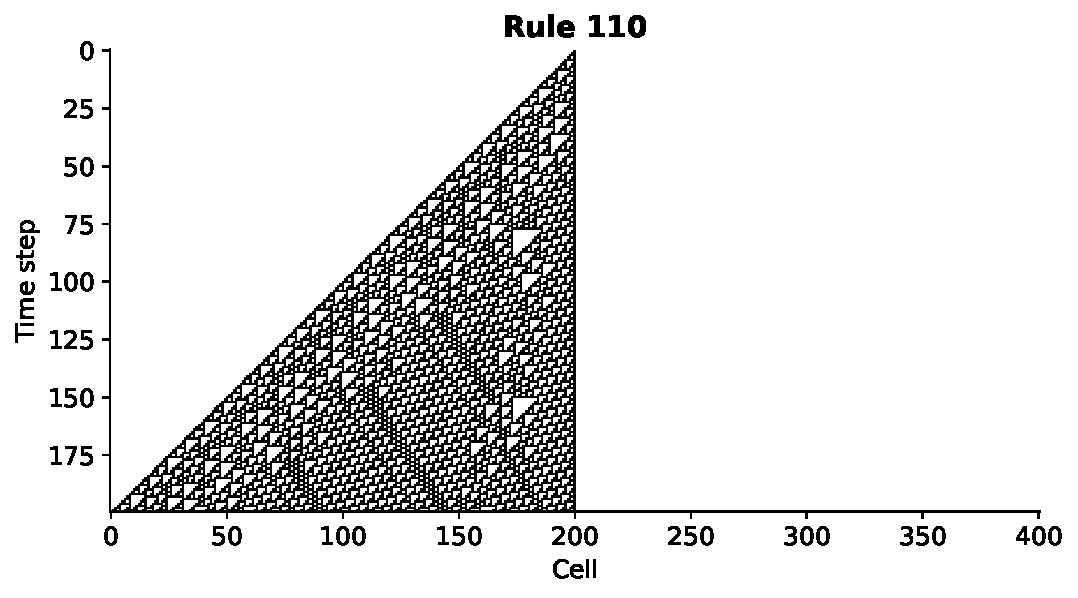
\includegraphics[width=\textwidth]{images/eca_rule110.pdf}
    \end{center}
    \column{0.5\textwidth}
    \begin{itemize}
      \item Rule 110 produces a mixture of \textbf{regular} and \textbf{complex} structures.
      \item Gliders, oscillators, and other structures interact.
      \item Proven \textbf{Turing complete} by Matthew Cook in 2004.
      \item This means a 1D, 2-state, 3-neighbour CA can simulate \textbf{any computer}.
    \end{itemize}
  \end{columns}
\end{frame}

\begin{frame}{Rule 90 --- Sierpinski Triangle}
  \begin{columns}
    \column{0.5\textwidth}
    \begin{center}
      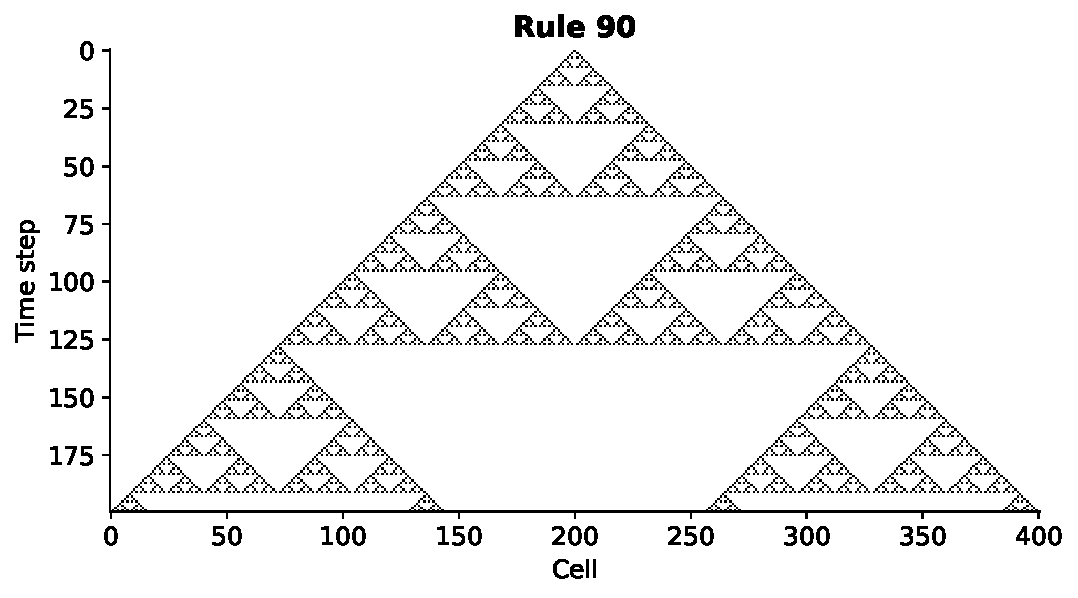
\includegraphics[width=\textwidth]{images/eca_rule90.pdf}
    \end{center}
    \column{0.5\textwidth}
    \begin{itemize}
      \item Rule 90 produces a perfect \textbf{Sierpinski triangle}.
      \item This is a well-known \textbf{fractal}.
      \item The rule is equivalent to \textbf{XOR} of the two neighbours.
      \item Connection to Lesson 5: fractals and chaos from simple rules.
    \end{itemize}
  \end{columns}
\end{frame}

\begin{frame}[fragile]{Implementing an Elementary CA}
  \begin{lstlisting}
def rule_to_table(rule_number):
    """Convert rule number to lookup table."""
    return {(i>>2 & 1, i>>1 & 1, i & 1):
            (rule_number >> i) & 1
            for i in range(8)}

def step_eca(row, table):
    """Apply one step of the ECA rule."""
    n = len(row)
    new = np.zeros(n, dtype=int)
    for i in range(n):
        left  = row[(i - 1) % n]
        center = row[i]
        right = row[(i + 1) % n]
        new[i] = table[(left, center, right)]
    return new
  \end{lstlisting}
\end{frame}

\begin{frame}{Exercise: Elementary Cellular Automata}
  \begin{enumerate}
    \item Implement the rule lookup table and the step function.
    \item Generate the space-time diagram for Rule 30, Rule 90, and Rule 110.
    \item Classify each rule according to Wolfram's four classes.
    \item Explore: which other rules produce interesting patterns? Try Rules 54, 60, 150, 184.
    \item Advanced: implement Rule 184 as a \textbf{traffic model} --- interpret 1 as a car and observe traffic jams.
  \end{enumerate}
\end{frame}
